\chapter{Experimental Setup}

In this chapter, I outline the datasets used in this work, the preprocessing applied to the audio and chord annotations, the evaluation metrics used to compare the models and details of the training process.

\section{Data}

I spent the initial period of this project finding a suitable dataset for training and testing. \citet{JAAH} use the \emph{JAAH} dataset while \citet{MelodyTranscriptionViaGenerativePreTraining} use the \emph{HookTheory} dataset. Many works use a combination of the \emph{McGill Billboard}, \emph{Isophonics}, \emph{RWC-Pop} and \emph{USPop} datasets. However, none have audio available. Furthermore, annotations come from different sources in different formats. I spent time looking at other sources audio data, pre-computed features of audio which are available for some datasets and compiling disparate annotations in different formats. I also contacted authors of previous ACR works to see if they could provide me with audio. I was able to get in contact with Andrea Poltronieri, a PhD student at the University of Bologna, one of the authors of the chord corpus or 'ChoCo' for short~\citep{Choco}. He provided me with labelled audio for the 1217 songs that are commonly used, alongside labelled audio for the \emph{JAAH} dataset. This was a great help despite it coming several weeks into the project.

I refer to the dataset used in this work as \emph{pop}. It consists of songs from the \emph{Mcgill Billboard}, \emph{Isophonics}, \emph{RWC-Pop} and \emph{USPop} datasets introduced in Section~\ref{sec:background-data}. This collection was initially proposed in work by \citet{FourTimelyInsights} to combine some of the known datasets for chord recognition. The dataset consists of subsets from the above sources filtered for duplicates and selected for those with annotations available. In total, there are 1,213 songs. The dataset was provided with obfuscated filenames and audio as \texttt{mp3} files and annotations as \texttt{jams} files~\citep{JAMS}. 

\newpage
\subsection{Data Integrity}\label{sec:data-integrity}

Several possible sources of error in the dataset are investigated below.

\textbf{Duplicates:} Files are renamed using provided metadata identifying them by artist and song title. This is done to identify duplicates in the dataset. There is only one: Blondie's \emph{One Way or Another}, which has two different recordings. It is removed from the dataset. Automatic duplicate detection is conducted by embedding each audio using mel-frequency cepstral coefficients (MFCC)~\citep{MFCC}. This function is commonly used to embed audio into low dimensions. This provides a fast and easy way of quantifying similarity. Audio is passed through the \texttt{mfcc} provided in \texttt{librosa}~\citep{librosa} with 20 coefficients. A song's embedding is calculated as the mean MFCC over all frames. Cosine similarities are then calculated for all pairs of tracks. None of the top 50 similarity scores yielded any sign of duplication. I proceed with the assumption that there are no further duplicates in the dataset.

\textbf{Chord-Audio Alignment:} It is pertinent to verify that the chord annotations align with the audio. Misaligned annotations could make training impossible. Ten songs are manually investigated for alignment issues by listening to the audio and comparing it to the annotations directly. The annotations are all well-timed with detailed chord labels.

Automatic analysis of the alignment of the audio and chord annotations is also done using the cross-correlation between the derivative of the CQT over time and the chord annotation. A maximum correlation at a lag of zero would indicate good alignment as the audio changes at the same time as the annotation. The derivative of the CQT in the time dimension is estimated using the \texttt{delta} function from \texttt{librosa}. The chord annotations are converted to a binary vector, where each element corresponds to a frame in the CQT and is 1 if a chord change occurs at that frame and 0 otherwise. Both the CQT derivatives and binary vectors are normalised by subtracting the mean and dividing by the standard deviation. Finally, cross-correlation is computed using the \texttt{correlate} function from \texttt{numpy}. A typical cross-correlation for a song is visualised in Appendix~\ref{app:cross_correlation}. The cross-correlation is periodic and repeats every 20 frames or so. Listening to the song, the period of repetition is a fraction of a bar length. 

To check alignment across the dataset, I plot a histogram of the lag of the maximum cross-correlations over songs in Figure~\ref{fig:durations-and-lags}. Under the assumption that the annotations are not incorrect by more than 5 seconds, the region of possible maximal lags is restricted to a window of 50 frames on either side of 0. This reduction does not change the shape of the picture. Instead, focusing on a reduced set of lags allows more detail to be visible. The majority of songs have a maximum lag close to 0, with a few outliers. This can be attributed to noise. A final check is done by looking at the difference in length of the audio files and chord annotations. A histogram of differences in length is also shown in the figure. The majority of songs have a difference in length of 0, with a few outliers almost all less than a second. This evidence, combined with the qualitative analysis, is convincing enough to leave the annotations as they are for training.

\begin{figure}[H]
    \centering
    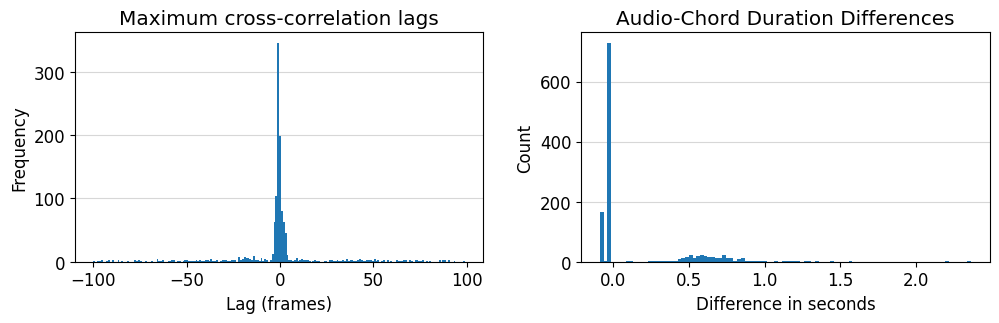
\includegraphics[width=1.0\textwidth]{figures/duration_diffs_and_lags.png}
    \caption{Histograms of the maximum cross-correlation lags and the difference in length between the audio and chord annotations. Both show results close to $0$, suggesting good alignment between audio and annotations. }\label{fig:durations-and-lags}
\end{figure}

\textbf{Incorrect and Subjective Annotations:} Throughout manual listening, no obviously wrong annotations were found. However, looking at songs on which the preliminary models perform the worst using the \texttt{mirex} metric, three songs stick out. `Lovely Rita' by the Beatles, `Let Me Get to Know You' by Paul Anka and `Nowhere to Run' by Martha Reeves and the Vandellas all had scores below $0.05$. In these songs, the model consistently guessed chords one semitone off, as if it thought the song was in a different key. Upon listening, it became clear that the tuning was not in standard A440Hz for the first two songs and the key of the annotation was wrong for the other. These songs were removed from the dataset. All reported results exclude these data points. No other songs were found to have such issues.

Chord annotations are inherently subjective to some extent. Detailed examples in \emph{pop} are given by \citet{FourTimelyInsights}. They also note the presence of several songs in the dataset of questionable relevance to ACR, as the music itself is not well-explained by chord annotations. However, these are kept in for consistency with other works as this dataset is often used in the literature. Some works decide to use the median as opposed to the mean accuracy in their evaluations in order to counteract the effect of such songs on performance~\citep{StructuredTraining}. We think that this is unnecessary as the effect of these songs is likely to be small and we do not wish to inflate our results inadvertently. Further evidence for the use of the mean is given in Section~\ref{sec:evaluation}.

\subsection{Preprocessing}

\subsubsection{Audio to CQT}\label{sec:audio-to-cqt}

I first convert the audio to a constant-Q transform (CQT) representation introduced in Section~\ref{sec:background-features}. CQTs are common in ACR and is used as a starting point for this work. The CQT was computed using \texttt{librosa}, using the built-in \texttt{cqt} function. A sampling rate of $44100$Hz was used, with a hop size of 4096, 36 bins per octave, 6 octaves and a fundamental frequency corresponding to the note \texttt{C1}. These parameters were chosen to be consistent with previous works~\citep{StructuredTraining} and with standard distribution formats. The CQT is returned as a complex-valued matrix containing phase, frequency and amplitude information. Phase information was discarded by taking the absolute value before being converted from amplitude to decibels (dB), equivalent to taking the logarithm.

The CQT matrix of a song has size $216 \times F$ where 216 is the number of frequency bins and $F$ is the number of frames in the song. The number of frames can be calculated as $F = \lceil \frac{44100}{4096} L  \rceil$ where $L$ is the length of the song in seconds, 44100 is the sampling rate in Hertz (Hz) and 4096 is the hop length in samples. A 3-minute song has just under 2000 frames. To save on computational cost, the CQT was pre-computed into a cached dataset rather than re-computing each CQT on every run.

\subsubsection{Chord Annotations}\label{sec:chord-annotations}

The chord annotation of a song is represented as a sorted dictionary, where each entry contains the chord label, the start time and the duration. The chord label is represented as a string in Harte notation~\citep{HarteNotation}. For example, C major 7 is \texttt{C:maj7} and A half diminished 7th in its second inversion is \texttt{A:hdim7/5}. The notation also includes \texttt{N}, a no chord symbol, and \texttt{X}, an unknown chord symbol.

Such a chord vocabulary is too flexible to be used as directly as a target for a machine learning classifier trained on limited data. It would contain thousands of classes, many of which would appear only once. Instead, I define a restricted chord vocabulary. This contains 14 qualities: major, minor, diminished, augmented, minor 6, major 6, minor 7, minor-major 7, major 7, dominant 7, diminished 7, half-diminished 7, suspended 2, and suspended 4. \texttt{N} denotes no chord playing and chords outside the vocabulary are mapped to \texttt{X}, a dedicated unknown symbol. Letting $C$ denote the size of the chord vocabulary, $C=12\cdot14 + 2 = 170$. This vocabulary is consistent with much of the literature~\citep{StructuredTraining,FourTimelyInsights,ACRLargeVocab1}. \citet{ACRLargeVocab1} use a more detailed vocabulary by including inversions, but I decide to remain consistent with other previous works. As \citet{StructuredTraining} note, $C=170$ is sufficient for the dataset to exhibit a significant imbalance in the chord distribution. Their methodology is easily extensible to larger vocabularies. If performance is not yet satisfactory on $C=170$, it is unlikely that performance will improve with a larger vocabulary.

Both training labels and evaluation labels are converted to this vocabulary. If the evaluation labels were kept in the original Harte notation, the model would be unable to identify them. The method for converting from Harte notation to a symbol in the chord vocabulary is similar to that used by \citet{StructuredTraining} and is detailed in Appendix~\ref{app:chord_mapping}.

A simpler chord vocabulary is also sometimes used. It contains only the major and minor quality for each root, and the \texttt{N} and \texttt{X} symbols. For example, \texttt{C:maj7} is mapped to \texttt{C:maj} while \texttt{A:hdim7/5} is mapped to \texttt{X}. For this vocabulary, $C=26$. I did some preliminary tests with this vocabulary but quickly found that model performance was similar over the two vocabularies. Results and analysis can be found in Appendix~\ref{app:small_vs_large_vocabulary}. Additionally, the \texttt{majmin} evaluation metric compares chords over this smaller vocabulary and is mentioned in Section~\ref{sec:evaluation}. The smaller vocabulary is not used in the rest of this work as there seems to be no advantage over the larger vocabulary.

Frames are allocated a chord symbol based on which chord is playing in the middle of the frame. While this may not be a perfect solution, frames are $\approx93$ms long, which is shorter than the minimum duration of a chord in the dataset. This guarantees that the chord label for every frame plays for at least half the frame. Furthermore, only $4.4\%$ of frames include a chord transition.

\subsection{Chord Distribution}

Much of the recent literature has focused on the long tail of the chord distribution, using various methods to address the issue. It is first helpful to understand the distribution of chords in the datasets, illustrated in Figure~\ref{fig:chord-distribution}. The distribution is broken down both by root and quality, using the chord vocabulary with $C=170$. The plots show that the distribution over qualities is highly skewed, with major and minor chords making up the majority of the dataset, and qualities like majorminor and diminished 7th chords, two or three orders of magnitude less common. The distribution over roots is far less skewed, although there is a preference for chords in keys with common roots like A, C and D.

\begin{figure}[H]
    \centering
    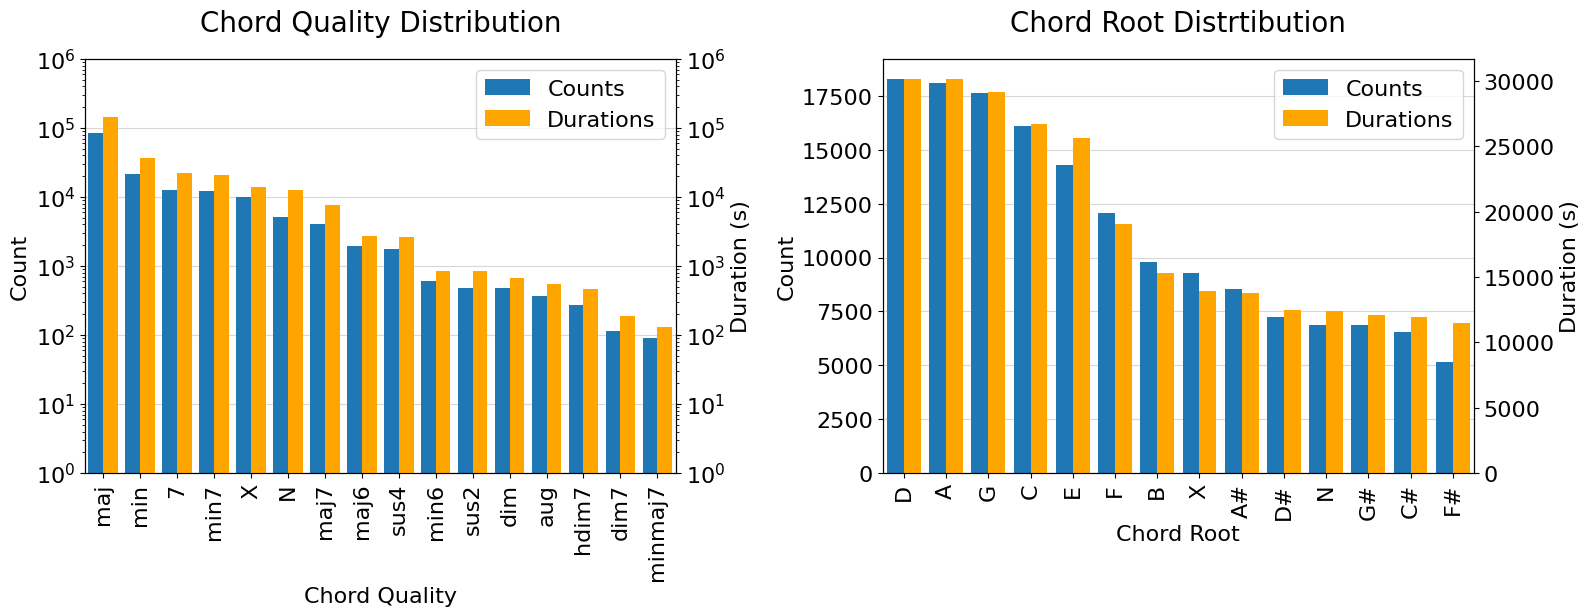
\includegraphics[width=1.0\textwidth]{figures/chord_distribution.png}
    \caption{Chord distributions over qualities (left) and roots (right) in the \emph{pop} dataset. The plots show the raw counts in frames and the duration in seconds for each chord root/quality. Note that the y-axis over qualities is in a logarithmic scale. The qualities are very imbalanced, with \texttt{maj} as the most popular. Conversely, roots are relatively balanced.}\label{fig:chord-distribution}
\end{figure}


% \subsection{JAAH Dataset}

% TODO: I was warned by Andrea that the JAAH dataset has not been as commonly used as dataset the Billboard dataset. Therefore he could not guarantee that the audio was aligned for this dataset.

% - As yet, JAAH is unused in this work
% - Data was received as \texttt{.flac} files which were first converted to \texttt{.mp3} files to be in line with the Billboard dataset
% - Comparison of the two datasets
% - Description of the JAAH dataset and its use in this work
% - Intended to be used as a test set to test the synthetic data generation.

\section{Evaluation}\label{sec:evaluation}

As is standard for ACR, I use weighted chord symbol recall (WCSR) to evaluate chord classifiers. Simply put, WCSR measures the fraction of time that a classifier's predictions are correct. I include a formal definition in Appendix~\ref{app:weighted_chord_symbol_recall_definitions}. Correctness can be measured in a variety of ways, such as \texttt{root}, \texttt{third} and \texttt{seventh}, which compare along roots, thirds, or sevenths respectively. I also use the \texttt{mirex} score, where a prediction is correct if it shares at least three notes with the label. This allows for errors like mistaking \texttt{C:7} for \texttt{C:maj}. Finally, I use \texttt{acc}, or simply accuracy, to denote the overall accuracy where symbols must match exactly.

Other measures of correctness are sometimes used. These include \texttt{majmin}, a measure of correctness over only major and minor qualities. I use this measure only to substantiate the use of the larger vocabulary in Appendix~\ref{app:small_vs_large_vocabulary}. Measures of correctness over triads and tetrads are also sometimes used, but these are highly correlated with \texttt{third} and \texttt{seventh}, respectively. This correlation is to be expected as the third and seventh are strong indicators of the triad and tetrad of the chord. This was verified empirically on preliminary experiments which are omitted.

All metrics are implemented in the \texttt{mir\_eval} library~\citep{mir_eval}, which also provides utilities for calculating WCSR from frame-wise chord predictions. The mean WCSR is computed over all songs in the evaluation set. Some other works report the median. Empirically, I found the median to be $\approx 2\%$ greater than the mean. This may be due to those songs identified as being unsuitable for chordal analysis by \citet{FourTimelyInsights}. I report only the mean throughout this work. This was chosen for being more commonly used in recent literature and because it is important for a metric to detect if the model performs poorly over certain genres.

For some experiments, two further metrics are calculated. These are the mean and median class-wise accuracies, called \texttt{acc}\textsubscript{class} and \texttt{median}\textsubscript{class}, respectively. \texttt{acc}\textsubscript{class} has previously been defined in terms of discrete frames by \citet{ACRLargeVocab1}. I redefine \texttt{acc}\textsubscript{class} here in terms of WCSR and introduce \texttt{median}\textsubscript{class}. The definitions can be found in Equations~\ref{eq:class_wise}.

\begin{equation}\label{eq:class_wise}
    \text{acc}\textsubscript{class} = \frac{1}{C} \sum_{c=1}^{C} \text{\emph{WCSR}}(c)
\quad \quad
    \text{median}\textsubscript{class} = \text{median}_{c=1}^{C} [\text{\emph{WCSR}}(c)]
\end{equation}

$C$ denotes the number of chord classes. $\text{\emph{WCSR}}(c)$ is the WCSR considering only time when chord $c$ is playing. A formal definition of $\text{\emph{WCSR}}(c)$ is also included in Appendix~\ref{app:weighted_chord_symbol_recall_definitions}.

These metrics are intended to measure the model's performance on the long tail of the chord distribution. Measuring both the mean and median is informative as it provides a sense of the skew in performance over classes. While the metric can be defined for any measure of correctness, I report only the \texttt{acc} as I found it to be the most informative. For example, the mean class-wise \texttt{root} score is harder to interpret.

The justification for redefining \texttt{acc}\textsubscript{class} this way is that metrics calculated over discrete frames are not comparable across different frame lengths and are dependent on the method of allocating chords to frames. Instead, continuous measures evaluate models based on the percentage of time that they are correct. This more closely reflect what we truly desire from the model. To illustrate this, imagine a very long frame length. The model could have perfect scores on these frames but be making terrible predictions for much of the song. Through preliminary experiments, it became clear that there are negligible differences between rankings between models in discrete and continuous measures for sufficiently small hop lengths. Nevertheless, I propose that the field of ACR adopts a continuous measure of class-wise accuracy.

I do not also compute \emph{quality}-wise accuracies as computed by \citet{CurriculumLearning}. Quality-wise metrics only ensure that each root is equally weighted. As roots are fairly balanced, this would not add much information. I therefore do not evaluate using quality-wise metrics.

For most experiments, the metrics on the validation set are used to compare performance. The test set is used only to compare the final accuracies of select models in Section~\ref{sec:test-set}.

Other evaluation tools are used such as confusion matrices and the number of chord transitions per song. Note that confusion matrices are calculated using discrete frames for ease of computation. In an ideal setting, these would also be calculated using continuous measures. Given the small differences between the two for short frame lengths, I decided it was not worth the additional engineering effort and computational cost.

\section{Training}\label{sec:training}

For the majority of experiments, I use a random 60/20/20\% training/validation/test over songs in the dataset. This split is kept constant across experiments. This contrasts much of the literature, which uses a 5-fold cross-validation introduced by \citet{FourTimelyInsights}. I did not maintain this status quo in order to obtain clean estimators of the generalisation error using the held-out test set and to save on computation time. For final testing, models are re-trained on the combined training and validation sets and tested on the test set.

Three variants of the dataset are used for training, validation and testing. For training, an epoch consists of randomly sampling a patch of audio from each song in the training set. The length of this sample is kept as a hyperparameter, set to $10$ seconds for the majority of experiments, based on values provided by \citet{StructuredTraining} and a hyperparameter search found in Section~\ref{sec:model_hyperparameters}. For evaluation, the entire song is used as performance was found to be marginally better. This is later discussed in Section~\ref{sec:crnn_performance_across_context}. When validating mid-way through training, songs are split into patches of the same length as the training patches to save on computation time. Samples in a batch are padded to the maximum length of a sample in the batch and padded frames are ignored for loss and metric calculation.

Experiments are run on two clusters with some further evaluation taking place locally. The first is The University of Edinburgh's ML Teaching Cluster. Here, NVIDIA GPUs are used, mostly GTX Titan Xs (12GB VRAM) and RTX A6000s (48GB VRAM) depending on availability on the cluster. Resources have inconsistent availability. Therefore, some experiments are run on Eddie, The University of Edinburgh's research compute cluster, on CPUs due to the lack of availability of GPUs.

Training code is implemented in \texttt{PyTorch}~\citep{pytorch} with seed set to $0$. Unless stated otherwise, models are trained with the Adam optimiser~\citep{adam} with a learning rate of $0.001$ and pytorch's \texttt{CosineAnnealingLR} scheduler, set to reduce the learning rate to 1/10th of its initial value over the run. Models are trained to minimise the cross entropy loss between the predicted chord and the true chord distribution. I use a batch size of 64 and train for 150 epochs unless stated otherwise. Validation part-way through training is conducted every 5 epochs in order to save time. The model is saved whenever the validation loss improves. Each training run takes approximately 30 minutes of GPU time or 1 hour 30 minutes of CPU time. This can vary up to 10 hours of CPU time for experiments with more expensive computations and larger input.